\subsection{Análisis de HW}

A continuación se analiza el esquemático y sus componentes con osciloscopios y multimetros para la verificación de su correcto funcionamiento.


Para poder visualizar el comportamiento de las señales se ajustó la escala del osciloscopio a $1s$. A continuación se presenta un fragmento de la señal del osciloscopio (lo más que se fue capaz de extender) la cual coincide con  el diagram de tiempo solicitado en figura \ref{diagrama_temporizacion}. La siguiente figura se encuentra en el estado D y muesta el estado A, B, C y D.

\begin{figure}[H]
\centering
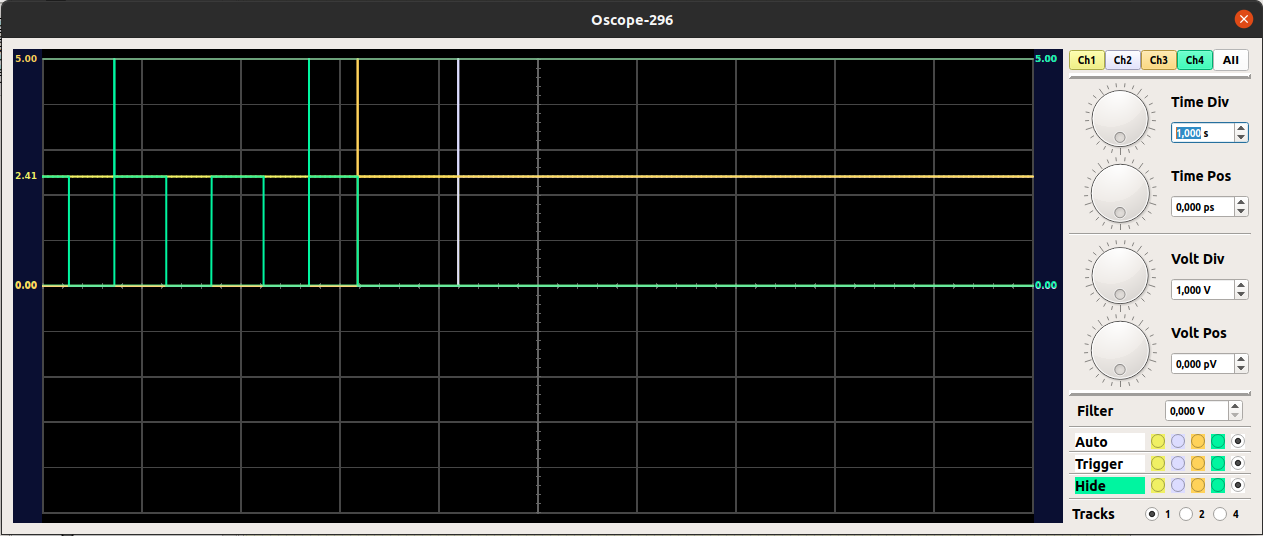
\includegraphics[scale=0.5]{./images/os.png} 
\caption{Framento de diagrama de tiempo.}
\label{f1}
\end{figure}

\begin{figure}[H]
\centering
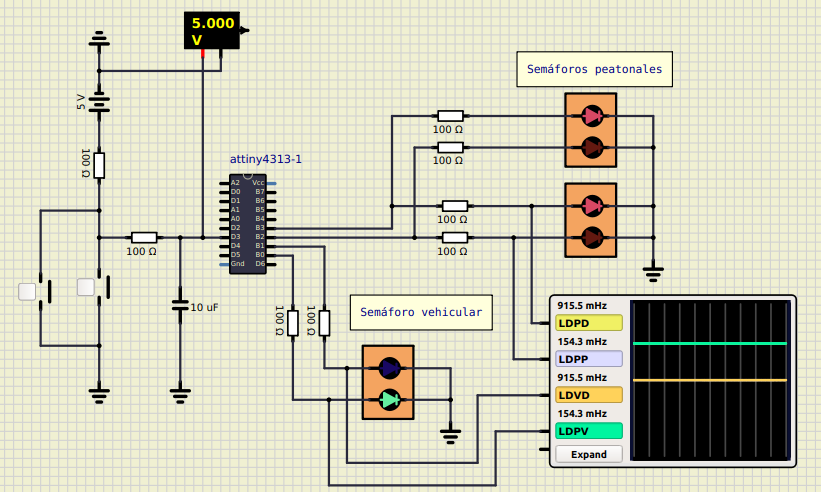
\includegraphics[scale=0.8]{./images/A.png} 
\caption{Circuito en estado A.}
\label{f1}
\end{figure}


\begin{figure}[H]
\centering
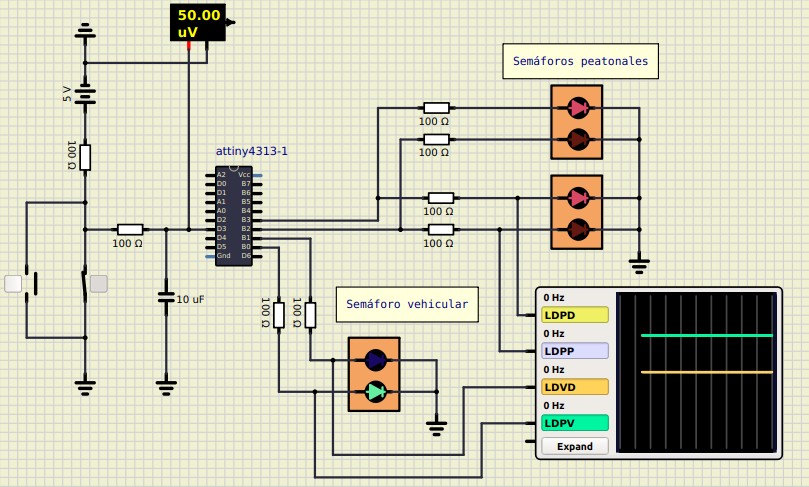
\includegraphics[scale=0.8]{./images/A1.png} 
\caption{Circuito en estado A justo en donde ocurre la interrupción o primera entrada.}
\label{f1}
\end{figure}

En la siguiente figura el LED encerrado en un cuadro verde está haciendo blink.
\begin{figure}[H]
\centering
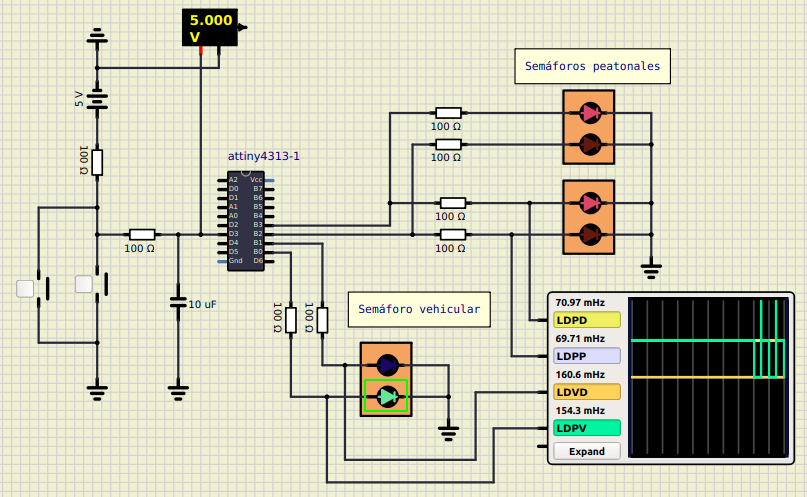
\includegraphics[scale=0.76]{./images/B.png} 
\caption{Circuito en estado B.}
\label{f1}
\end{figure}


\begin{figure}[H]
\centering
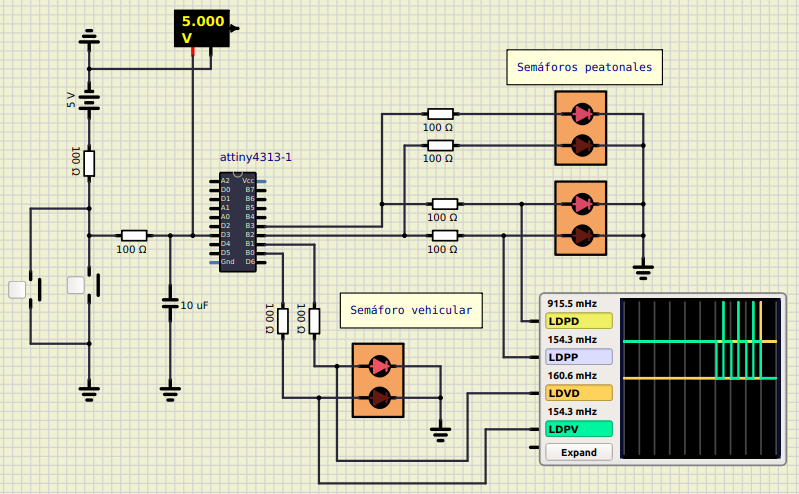
\includegraphics[scale=0.76]{./images/C.png} 
\caption{Circuito en estado C.}
\label{f1}
\end{figure}


\begin{figure}[H]
\centering
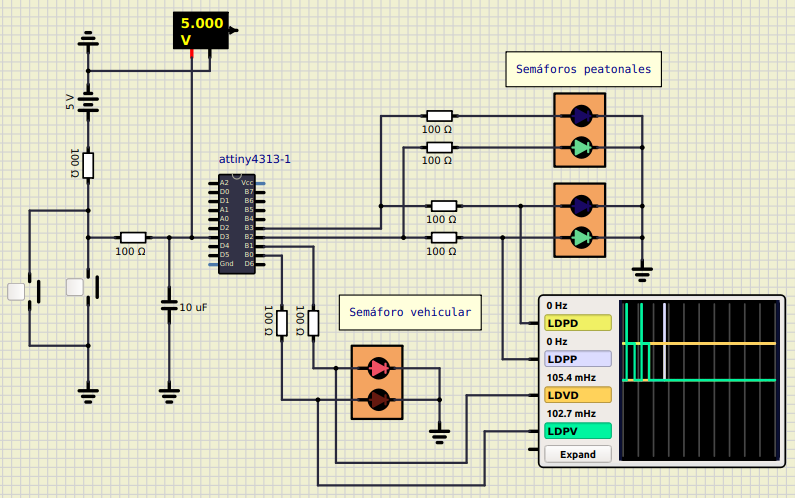
\includegraphics[scale=0.76]{./images/D.png} 
\caption{Circuito en estado D.}
\label{f1}
\end{figure}


En la siguiente figura los LEDs encerrados en un cuadro verde están haciendo blink.
\begin{figure}[H]
\centering
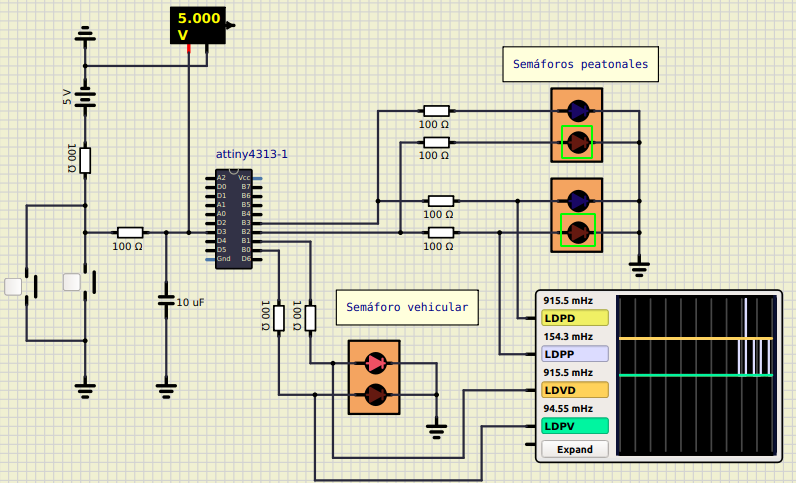
\includegraphics[scale=0.76]{./images/E.png} 
\caption{Circuito en estado E.}
\label{f1}
\end{figure}